\section{3G og GPS modul}

I dette afsnit beskrives valg af 3g og GPS modul. 

\subsection{3G modul}
For at kunne kommunikere mellem webapplikation og drone er det nødvendigt at dronen har forbindelse til internettet. 
Der kræves en hurtig og stabil internetforbindelse, da dronen under flyvning både skal sende billeder og modtage kommandoer fra webapplikation.

Til at sende informationer mellem webapplikation og dronen er det bestemt som minimum at anvende GPRS protokollen eller højere. Nedenfor ses en tabel der viser de hastigheder fra forskellige mobilnet protokoller. 

\begin{figure}[H]
\centering
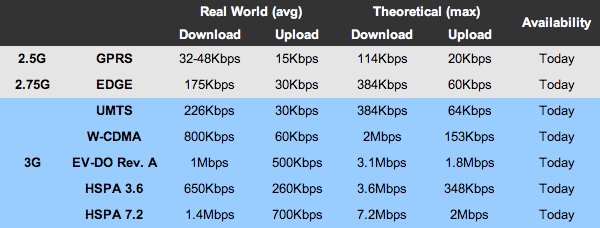
\includegraphics[width=0.7\textwidth]{Billeder/3g-table.png}
\caption[trådløs_teknologi]{trådløs teknologi\protect\footnotemark}
\label{fig:3gtable}
\end{figure}
\footnotetext{http://www.techspot.com/guides/272-everything-about-4g/}


Valg af mobilnetværks modul er foretaget ud fra følgende kriterier:
\begin{itemize}
	\item Datarate.
	\item Pris.
\end{itemize}

Ud fra kriterierne fandt gruppen frem til følgende to moduler der kunne anvendes:

Sparkfuns\footnote{https://www.sparkfun.com/products/9607} Cellular Shield. Dette shield kan bruges sammen med en arduino, hvor det fungerer som et shield der skal placeres på arduinoen. Dog understøtter dette shield kun mobilnet op til GPRS. Som vist på Figur~\ref{fig:3gtable} kan GPRS kun uploade med 20 Kbps teoretisk og nok nærmere $\sim$15 Kbps reelt.

Cooking-Hacks har lavet et 3G shield der er kompatibelt med arduino\footnote{http://www.cooking-hacks.com/documentation/tutorials/arduino-3g-gprs-gsm-gps}. Dette shield understøtter brugen af 3G, hvilket giver upload hastighed op til $\sim$2Mbps teoretisk og $\sim$700Kbps reelt set - se Figur~\ref{fig:3gtable}.

\begin{table}[H]
	\centering
		\begin{tabular}{|p{3.5cm}|p{5 cm}|p{5 cm}|} 
		\hline
			\textbf{ } & \textbf{Sparkfuns} 	& \textbf{Cookings-Hacks} \\ \hline
					Pris& 99 \$  & 149 \$ \\ \hline			 					 			
		\end{tabular}
	\caption{Prisoversigt moduler}
	%\label{tab:TC1}
\end{table}

\newpage

Begge shields har mulighed for at transmittere data mellem dronen og webapplikationen. Cookings Hacks' 3G shield er dog en bedre løsning, da det understøtter et nyere mobilt netværk, der giver mulighed for at sende og modtage data med større datarater.
Ved sammenligning af prisen ses, at Cooking Hacks shieldet koster mere end Sparkfuns, dog har Cooking Hacks shieldet den fordel at den udover 3G også indeholder GPS.

\subsection{GPS}
På grund af Cooking Hacks' 3G modul har indbygget GPS, blev det besluttet at benytte netop dette shield. Når GPS delen af shieldet bruges, kan det benyttets i tre forskellige modes: \textit{mobile-assisted, mobile-based og standalone}. \\
De forskellige modes gør det muligt at bruge GPS sammen med eller uden netværk. Hvis GPS'en anvendes sammen med netværk, bliver GPS koordinaterne bearbejdet og sendt til den ønskede enhed, mens den i \textit{standalone} giver koordinaerne direkte fra satellitterne.

\begin{figure}[H]
\centering
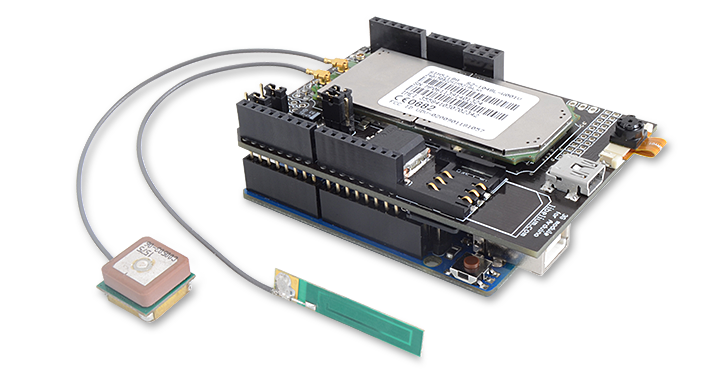
\includegraphics[width=0.7\textwidth]{Billeder/3G.png}
\caption{3G/GPS shield - fra cooking hacks\protect\footnotemark}
\label{fig:3gshield}
\end{figure}
\footnotetext{http://www.cooking-hacks.com/3g-gprs-shield-for-arduino-3g-gps}


På baggrund af undersøgelsen blev det besluttet at anvende 3G/GPS shield fra Cookings-Hacks til projektet. For det første er det billigere at købe 3G og GPS som et samlet modul end at købe 3G og GPS hver for sig. Desuden gør det en eventuel sammenkobling af 3G og GPS lettere.











